\documentclass[border=5pt]{standalone}
\usepackage{tikz}
\usepackage{amsmath}
\usetikzlibrary{arrows.meta}

\begin{document}
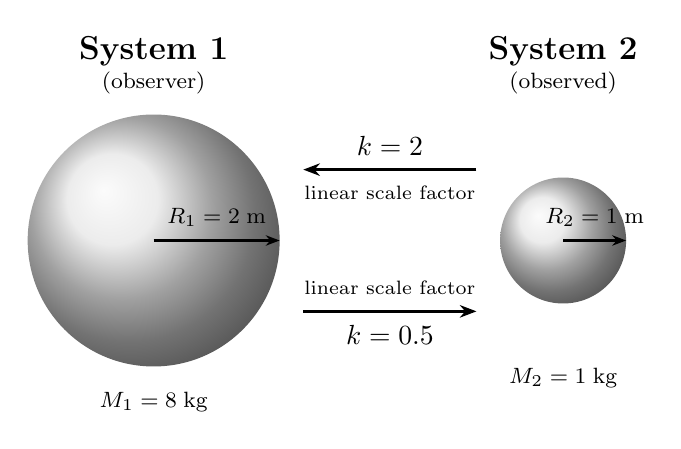
\begin{tikzpicture}

% System 1 (observer) — large sphere, left
\shade[ball color=gray!20] (-2.6,0) circle (1.6cm);
\node[font=\large\bfseries] at (-2.6,2.4) {System 1};
\node[font=\footnotesize] at (-2.6,2.0) {(observer)};
\draw[-{Stealth[length=5pt]}, thick] (-2.6,0) -- (-1.0,0);
\node[font=\footnotesize, above] at (-1.8,0.05) {$R_1 = 2\;\text{m}$};
\node[font=\footnotesize] at (-2.6,-2.05) {$M_1 = 8\;\text{kg}$};

% System 2 (observed) — small sphere, right
\shade[ball color=gray!20] (2.6,0) circle (0.8cm);
\node[font=\large\bfseries] at (2.6,2.4) {System 2};
\node[font=\footnotesize] at (2.6,2.0) {(observed)};
\draw[-{Stealth[length=5pt]}, thick] (2.6,0) -- (3.4,0);
\node[font=\footnotesize, above] at (3.0,0.05) {$R_2 = 1\;\text{m}$};
\node[font=\footnotesize] at (2.6,-1.75) {$M_2 = 1\;\text{kg}$};

% Scale factor: System 2 scaled up by k to System 1
\draw[-{Stealth[length=6pt]}, line width=1.2pt] (1.5,0.9) -- (-0.7,0.9);
\node[font=\normalsize\bfseries, above] at (0.4,0.95) {$k = 2$};
\node[font=\scriptsize] at (0.4,0.6) {linear scale factor};

% Scale factor: System 1 scaled down by k to System 2 (reverse perspective)
\draw[-{Stealth[length=6pt]}, line width=1.2pt] (-0.7,-0.9) -- (1.5,-0.9);
\node[font=\normalsize\bfseries, below] at (0.4,-0.95) {$k = 0.5$};
\node[font=\scriptsize] at (0.4,-0.6) {linear scale factor};

\end{tikzpicture}
\end{document}
